\documentclass{article}

% Set page size and margins
% Replace `letterpaper' with `a4paper' for UK/EU standard size
\usepackage[letterpaper,top=2cm,bottom=2cm,left=3cm,right=3cm,marginparwidth=1.75cm]{geometry}

\usepackage{amsmath}
\usepackage{graphicx}
\usepackage[colorlinks=true, allcolors=blue]{hyperref}
\usepackage[utf8]{inputenc}
\usepackage[russian]{babel}

\title{СВТ, Домашнее задание №1}
\author{Агеев Николай, 303 группа}

\begin{document}
\maketitle

\section{Описание задачи}

Требуется численно решить одномерную краевую задачу Дирихле для уравнения Лапласа:
$$
\begin{cases}
-u''(x) = f(x), \quad x \in (0; 1) \\
u(0) = a, \: u(1) = b
\end{cases}
$$

Протестировать программу требуется на функции $u(x) = \sin x$. Таким образом, правая часть в системе равна $f(x) = -u''(x) = \sin x$.

\section{Описание метода}

\subsection{Аппроксимация уравнения Лапласа}

Решение краевой задачи нужно искать с помощью метода конечных разностей. 
На отрезке $[0; 1]$ вводится равномерная сетка $\{x_0, x_1, \ldots, x_N\}$, где $x_i = ih$, $h = 1 / N$ - шаг сетки. Вводятся дискретные неизвестные $y_i = u(x_i), \ i = 0, 1, 2, ... , N$. В каждой точке $x_i, \ i = 1, ... , N - 1$ вторая производная функция приближается формулой конечных разностей по трём точкам:
$$
u''(x_i) \approx \frac{y_{i - 1} - 2y_i + y_{i + 1}}{h^2}
$$
Таким образом получается дискретная аппроксимация уравнения:
$$
-\frac{y_{i - 1} - 2y_i + y_{i + 1}}{h^2} = f(x_i)
$$

\subsection{Решение системы}

С учётом граничных условий система для дискретного решения принимает вид
$$\frac{1}{h^2}
\begin{bmatrix}
2 & -1 & & & & \\
-1 & 2 & -1 & & & \\
& -1 & 2 & -1 & & \\
& & & \ldots & & \\
& & & -1 & 2 & -1 \\
& & & & -1 & 2 \\
\end{bmatrix} = \begin{bmatrix}
y_1 \\
y_2 \\ 
y_3 \\
\ldots \\
y_{N-2} \\
y_{N-1} \\
\end{bmatrix} = \begin{bmatrix}
f(x_1) + a / h^2 \\
f(x_2) \\ 
f(x_3) \\
\ldots \\
f(x_{N-2}) \\
f(x_{N-1}) + b / h^2 \\
\end{bmatrix} $$

Данная система с трёхдиагональной матрицей решается методом прогонки.

Компоненты искомого вектора $y$ связаны соотношениями
$$y_i = \alpha_{i+1} y_{i+1} + \beta_{i+1}, \quad i = N-1, N-2, \dots, 1.$$

Из подстановки этих соотношений в систему находятся следующие соотношения:
$$
\alpha_{i} = \frac{-B}{A \alpha_{i - 1} + C}
$$
$$
\beta_{i} = \frac{f_i - A \beta_{i - 1}}{A \alpha_{i - 1} + C}
$$
, где $A, B$ и $C$ - значения на нижней, верхней и главной диагоналях соответственно (в конкретной задаче $A = B = -1, \ C = 2$).

Таким образом, путём вычисления чисел $\alpha_1, ... , \alpha_{n - 1}$ и $\beta_1, ... , \beta_{n - 1}$ в прямом порядке, а затем - чисел $y_{n - 1}, ... , y_1$ в обратном порядке, можно решить вышеописанную систему с трёхдиагональной матрицей.

\section{Результаты}

На построенном графике можно увидеть зависимость C-нормы и дискретной L2-нормы ошибки решения от числа отрезков сетки $N$.

\begin{figure}[!hq]
    \centering
    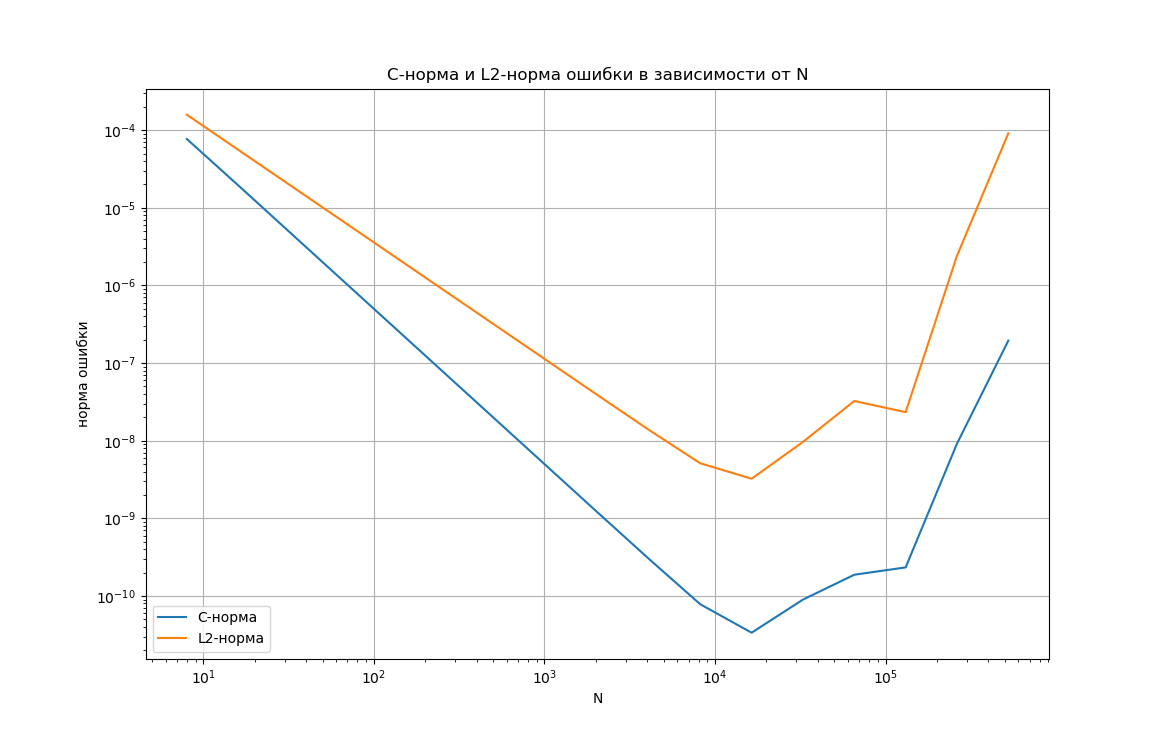
\includegraphics[width=1.0\linewidth]{graphic.png}
    \caption{Зависимость C-нормы и дискретной L2-нормы ошибки решения от $N$}
    \label{fig:graphic}
\end{figure}

\newpage

\begin{table}[!hq]
    \centering
    \begin{tabular}{|c|c|c|}
        \hline
        N & C-норма & L2-норма \\ \hline
  8 & 7.711480319994024e-05 &  0.00015853731268067868 \\ \hline
  16 & 1.9527005310160384e-05 &  5.6025866704240535e-05 \\ \hline
  32 & 4.881036226200841e-06 &  1.9805395130868587e-05 \\ \hline
  64 & 1.2202947158312938e-06 &  7.0020117296487744e-06 \\ \hline
  128 & 3.0514463944530945e-07 &  2.4755623564508607e-06 \\ \hline
  256 & 7.628601383924405e-08 &  8.752417478909127e-07 \\ \hline
  512 & 1.907150082303133e-08 &  3.094446602983054e-07 \\ \hline
  1024 & 4.7678090364655645e-09 &  1.0940435300766819e-07 \\ \hline
  2048 & 1.1923435572214203e-09 &  3.869228273675233e-08 \\ \hline
  4096 & 3.0025071318107166e-10 &  1.3779491004256964e-08 \\ \hline
  8192 & 7.818268255022076e-11 &  5.123022464215595e-09 \\ \hline
  16384 & 3.362587985833443e-11 &  3.2387394519678575e-09 \\ \hline
  32768 & 8.972789178329776e-11 &  9.649261583665113e-09 \\ \hline
  65536 & 1.8768331333518518e-10 &  3.2491817544386773e-08 \\ \hline
  131072 & 2.3339774557484816e-10 &  2.332949725552739e-08 \\ \hline
  262144 & 9.160457725698734e-09 &  2.414226184246755e-06 \\ \hline
  524288 & 1.947166099469655e-07 &  9.131482374945842e-05 \\ \hline
    \end{tabular}
    \caption{Зависимость C-нормы и дискретной L2-нормы ошибки решения от $N$}
    \label{tab:table}
\end{table}

На из графика и таблицы видно, что обе нормы ошибки решения уменьшаются с ростом числа отрезков сетки, но начиная с $N = 16384$ ошибка растёт. Это происходит из-за большого роста числа обусловленности трёхдиагональной матрицы, с которой  решается система.

\section{Выводы}

Написаны функции для численного решения уравнения Лапласа, протестированы на функции $u(x) = \sin x$, построены графики норм ошибок и приведена таблица со значениями ошибок на разном числе отрезков сетки.

\end{document}